% siminos/atlas/chart.tex  pdflatex atlas
% $Author$ $Date$

\section{Charting the \reducedsp: Global atlas}
\label{s:chart}

The \mslices\ as implemented here associates a `\slice' hyperplane to each
\template. As the inertial manifold is a highly contorted, nonlinear
curved manifold embedded in the $\infty$-dimensional \statesp, any such
linearization is good only locally: a single {\template} cannot be a good
match  globally.
    %
%  \includegraphics[width=1.00\textwidth,clip=true]{slicePhil0}

    \begin{itemize}
      \item flow in a \slice: \cLf\ example
      \item {\chartBord}: \cLf\ example
      \item 2-chart atlas, ridges:  \cLf\ example
      \item gauge fixing, geometric phase?
    \end{itemize}


\APW{111104 The first sentence requires simplifying!}
As group orbits % of compact Lie groups
are smooth manifolds (in case at hand, 2-tori), have natural linear
representations (under linear action of a symmetry group, \statesp\
decomposes into a sum over irreducible subspaces), and have natural local
coordinate frames (the group tangent, curvature Frenet-Serret frames
\refeq{FrenetFrame}), good \slice s should be easier to construct than
the elusive ``good'' Poincar\'e sections of the time-evolution flows.
Indeed, as a generic \slice\ \refeq{PCsectQ0} is the set of all
group-orbit points closest to a given {\template}, it slices the group
orbits of \emph{all} full \statesp\ points\rf{FrCv11}. However, for a
nonlinear flow, there is no single \slice\ that really does the job: our
\slice\ is locally a hyperplane, expected to be a good description of
solutions similar to a given {\template} in some open neighborhood. The
variational distance condition \refeq{PCsectQ0} is only an extremum
condition, and as the group orbits of highly nonlinear states are highly
contorted (see \reffig{fig:2830GO6}\,(b)), they can have many
extrema, and multiple sections by a \slice\ hyperplane. For example, an
\rpo\  torus is always intersected by a \slice\ hyperplane in two or more
sections, see \reffig{fig:sliceimage}.
    \PC{\refFig{fig:sliceimage}, new proposal: take points on the good,
    blue \po, run each along the group orbit until $\sspRSing \in S$
    where it intersects the \sset, see \refeq{sspRSing}, and thus plot
    the border of where the local slice ends, once on the left, and once
    on the right of the {\template}. Catch - I have not thought this
    through, not sure that the condition \refeq{sspRSing} can be
    satisfied on every group orbit...
    }

%%%%%%%%%%%%%%%%%%%%%%%%%%%%%%%%%%%%%%%%%%%%%%%%%%%%%%%%%%%%%%%%%%%%%
\begin{figure}
   \centering
   %\includegraphics[width=0.45\textwidth]{2841GO3S}
   \caption{\label{fig:sliceimage}
      Every slice hyperplane cuts every group orbit at least twice (see
      \reffig{fig:slice}), once at       orbit's closest passage to the
      {\template}, with positive curvature \refeq{eq:curv},   and another
      time at the most distant passage, also satisfying the slice
      condition \refeq{eq:slcond}, but with negative curvature. An
      $\SOn{2}$ \rpo\ is topologically a torus, so the two cuts are the
      two \po\ images of the same \rpo, the good close one, and the bad
      distant one, on the other side of {\sset}, and thus not in the
      slice. Here this is illustrated by close cut (blue) of the \rpo\
      $\RPO{36.92}$ torus, \reffig{f:MeanVelocityFrame}\,({\it b}),
      plotted together with the most distant cut (red), in the same slice
      hyperplane, but not in the slice.
   }
\end{figure}
%%%%%%%%%%%%%%%%%%%%%%%%%%%%%%%%%%%%%%%%%%%%%%%%%%%%%%%%%%%%%%%%%%%%%


Fortunately, we do have a sharp definition of how far the neighborhood
of a {\template} extends:
a hyperplane captures faithfully neighboring group orbits as long
as it \slice s them transversally; it fails the moment the group tangent of
a not-so close point $\sspRSing$ lies in the \slice.
At this instant the group tangent is orthogonal to the \slice\ tangent,
\beq
\braket{\groupTan(\sspRSing)}{\sliceTan{}}= 0
\, ,
\ee{sspRSing}
%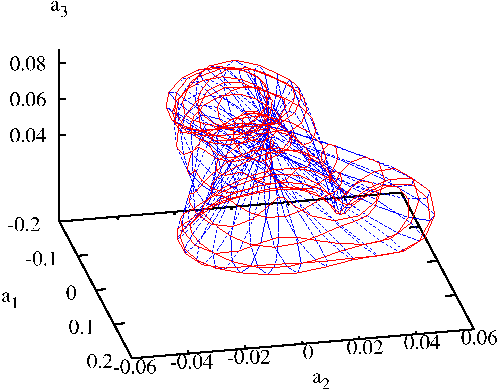
\includegraphics[width=1.20\textwidth]{2840GOt135M1} %{2830GO7}
%  \caption{\label{fig:2830GO6}
    %\label{fig:M1groupOrb}
%
and the phase velocity $\dot{\gSpace}(\sspRSing)$ in \refeq{reconstrEq}
diverges.  For points more distant the group orbits have more than one
intersection with the \slice\ hyperplane. It is clear what the trouble
with any single \slice\ hyperplane is: our slice condition and \slice s
are linear.

The physical task is to, for a given dynamical flow, pick a set of
qualitatively distinct {\template s} (for example, one typical of 2-roll
states, one for 4-roll states, and so on) whose \slice s  are locally
transverse to open sets of nearby orbits, and which together provide a
good global atlas of $\pS/\Group$. Each \slice\ $\pS{}^{(j)}$, provides a
local chart at $\slicep{}^{(j)}$ for a neighborhood of an important,
qualitatively distinct class of solutions. Together they `Voronoi'
tessellate  the curved manifold in which the symmetry-reduced strange
attractor is embedded by a finite set of hyperplane tiles.
For further discussion, see \refappe{appe:slice}.

Coupled with our \statesp\ visualizations allows for explorations of
high-dimensional flows that hitherto were unthinkable. Symmetry reduction
is here achieved, and now all invariant solutions can be plotted
together, as one happy family: all points equivalent by symmetries are
represented by a single point, families of solutions are mapped to a
single solution, \reqva\ become \eqva, and \rpo s become \po s. Without
symmetry reduction, no full understanding of pipe and plane \pCf s is
possible.
    %
    \PC{2011-10-18 incorporate this paragraph:``
Note also that the rotation of a fluid flow into a \slice\ {\em is not}
an average over the 3D pipe azimuthal angle, it is the full snapshot of
the flow embedded in the $\infty$-dimensional \statesp. Symmetry
reduction is not a dimensional-reduction scheme, or flow modeling by
fewer degrees of freedom: the \reducedsp\ is also $\infty$-dimensional
and no information is lost, one can go freely between solutions in the
full and reduced \statesp s by integrating the associated
\emph{reconstruction equations}.
''}

\subsection{Global atlas}
% Predrag 2012-03-04: transferred here text from slice.tex

A \slice\ hyperplane captures faithfully neighboring group orbits until,
for a point $\sspRSing$ not so close to the \template\ its tangent vector
lies in the \slice,
\[
\braket{\groupTan(\sspRSing)}{\sliceTan{}}= 0
\,,
\]
and its group orbit is grazed tangentially rather than sliced transversally.
The {\phaseVel} $\dot{\gSpace}(\sspRSing)$ in
\refeq{reconstrEq} then diverges. Equivalently,
one can say that a \slice\ is transverse to a group orbit as long as its
curvature normal vector \refeq{eq:curv} is not normal to the {\template} vector,
\[
\braket{\groupTan(\sspSing)}{\sliceTan{}}
 =
-\braket{\Lg^2\sspSing}{\slicep}
 =
-\braket{\kappa(\sspSing) \,{\bf n}(\sspSing)}{\slicep}
 = 0
\,.
\]
This is also a linear condition, and it defines a hyperplane of points
\sspSing\ normal to  the quadratic Casimir-weighted curvature vector
$\kappa(\slicep) \, {\bf n}(\slicep)$, such that from the {\template} vantage
point their group orbits are not transverse, but locally `horizontal.'
%$(d\!-\!2)$\dmn\
{\Sset} $S$ is the locus of inflection points, a hyperplane through which
curvature of the distance function changes sign:
    \PC{demonstrate this}
set of all points
$\sspRSing$ which are both in the {\slice}, and whose group tangent
$\groupTan(\sspRSing)$ is also in the  {\slice},
    \PC{add Froehlich figure of {\Sset} $S$?}
    % 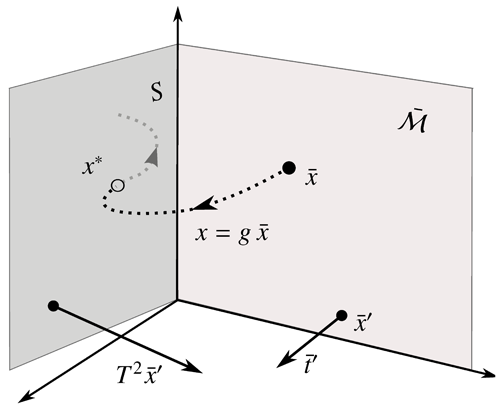
\includegraphics[width=0.80\textwidth]{inflectHype.png}
\beq
\braket{\sspRSing}{\sliceTan{}} \,=\, 0
    \,, \mbox{ and }
\braket{\groupTan(\sspRSing)}{\sliceTan{}}
 \,=\,
-\braket{\sspRSing}{\kappa(\slicep) \, {n}(\slicep)}
 =0
\,.
\label{sliceSingl0}
\eeq
A hyperplane segment of a \slice\ is good only up to the \sset. However,
the divergence in {\phaseVel} \refeq{reconstrEq} is an artifact of the
symmetry reduction by tangent hyperplanes, and thus an avoidable
nuisance.

Locally, our initial \slice\ chart $\pSRed{}^{(1)}$ is a ($d\!-\!1$)\dmn\
hyperplane. If we pick another {\template} point $\slicep{}^{(2)}$, it
comes along with its own \slice\ hyperplane $\pSRed{}^{(2)}$. Any
neighboring pair of $(d\!-\!1)$\dmn\ local \slice\ hyperplanes intersects
in a `ridge',
% (`boundary,' `edge'),
a $(d\!-\!2)$\dmn\ hyperplane, easy to compute.

Thus, in order to chart the \statesp\ of a turbulent flow, a set
of local \slice\ hyperplanes is needed to capture all of the asymptotic
dynamics. The choice of local \slice s should reflect the dynamically
dominant patterns seen in the solutions of nonlinear PDEs. We construct a
global atlas of the dimensionally \reducedsp\ $\pSRed = \pS/\Group$ by
deploying local linear \slice s  $\pS{}^{(j)}$ across neighborhoods of
the qualitatively most important \template\ {\cohStr s}
$\slicep{}^{(j)}$. For example, in reducing turbulent trajectories of
\refsect{s:rpos}, we use a set of \reqva\ as our \template s, see
\reffig{fig:thetadot2}. This is the periodic-orbit implementation of the
idea of {\statesp\ tessellation}.
% 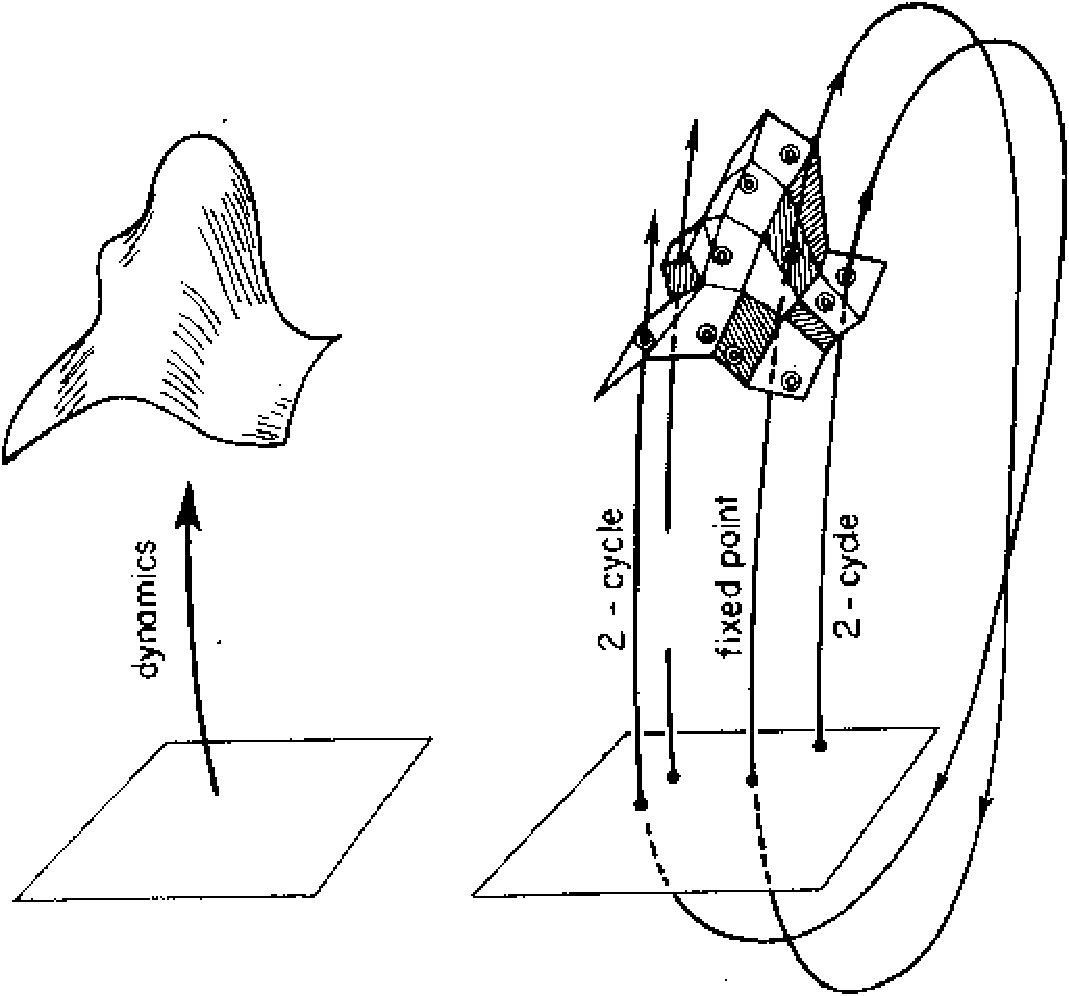
\includegraphics[width=0.60\textwidth]{f_1_08_1}
%%%%%%%%%%%%%%%%%%%%%%%%%%%%%%%%%%%%%%%%%%%%%%%%%%%%%%%
%   PC 2011-09-07 the two figures from the blog,
%    Channelflow.org/dokuwiki/doku.php?id=chaosbook:pipes,
%    2210switching.png and 2206\_thetadot.png}
%   replace by better something
\begin{figure}
  \centering
%  \includegraphics[width=0.75\textwidth]{2936Switch2}
  \caption{\label{fig:thetadot2}
Comparison of symmetry-reduced trajectory using a single {\template} ML
(blue, short-dash) with the same trajectory symmetry reduced using a set
of \template s (red, solid) indexed by $j(\zeit)$ (1 laminar; 2 LB; 3 ML; 4
MU; 5 UB; 6 S2a; 7 S2b), with {\template} at time $\zeit$ indicated on left
ordinate by (green, long-dash) line. Right ordinate: the shift deviation
from the mean shift, $\shift(\zeit)-\timeAver{\dot{\shift}}\,\zeit$,
where $\timeAver{\dot{\shift}}=1.274$ is estimated by a long-time
simulation. Both symmetry reductions begin with the same {\template} and
experience the same jumps in the shift starting at $\zeit\approx 40$. By
starting to switch the \template s at $\zeit\approx 60$, further jumps
(seen for the blue, short-dash line) are avoided (red, solid line).
  }
\end{figure}

The physical task is to, for a given dynamical flow, pick a set of
qualitatively distinct {\template s} whose \slice s  are locally
transverse to an open set of nearby orbits. Each \slice\ $\pS{}^{(j)}$,
provides a local chart at $\slicep{}^{(j)}$ for a neighborhood of an
important, qualitatively distinct class of solutions (2-rolls states,
3-rolls states, \etc). Together they `Voronoi' tessellate  the curved
manifold in which the symmetry-reduced strange attractor is embedded by a
finite set of hyperplane tiles. We have no advice on how to
systematically pick the individual \template s, other than that the
associated \slice\ tiles should be sufficiently small to exclude
group-orbit tangencies, \ie, stop before crossing their inflection
hyperplanes \refeq{sliceSingl0}.
